\section{Model of the quadricopter}

\subsection{Testing environment}
We have been doing experiments with Iris Plus 3DR\trademark quadricopters in the testing environment of the Smart Mobility Lab of KTH.
The environment is a $5\times5$ meter based area of 2 meters high.
Position of the agents are measured with the motion capture Qualisys\trademark.
The computation of the discrete controller is done offline.

\begin{figure}
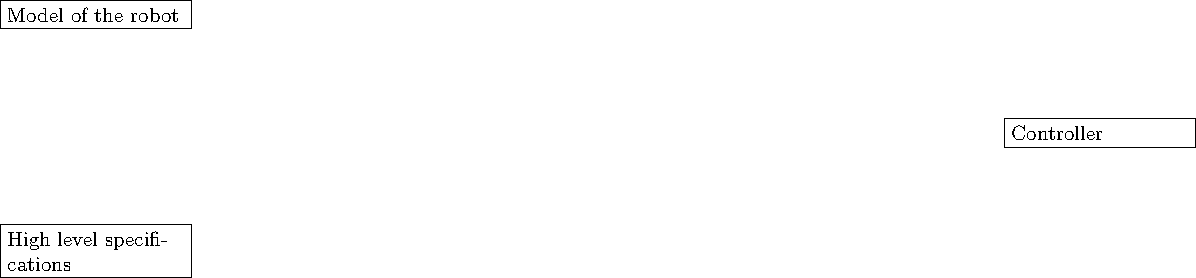
\includegraphics[width=\linewidth]{diagram.tex}
\end{figure}

\subsection{Model of the quadricopter}
We have been considering each quadricopter as 
Each dynamics of the quadricopter is decoupled from the other.
The chosen is a second integrator with velocity feedback. 

Modelisation of one axis

\subsection{Model of one axis}
We will use the second integrator model with a discrete set of controls.

\begin{equation}\label{eqn:lin_sys}
\begin{split}
\dot{\mathbf{x}} &= A \mathbf{x} + B \mathbf{u} + \mathbf{w}\\
\mathbf{y} &= C\mathbf{x}
\end{split}
\end{equation}
with
\begin{equation*} \label{eqn:sec_int}
A = \begin{bmatrix}
0 & 1\\ 
0 & -k
\end{bmatrix}
\textrm{, }
B = \begin{bmatrix}
0 \\ 
k 
\end{bmatrix}
\textrm{, }
k \in \mathbb{R}_+^\star
\end{equation*}

We will study the effect of the reduction over the size of the abstraction. In the case of the second integrator, we will observe both the position and the velocity of the agent:
\begin{equation}
C_{dble} = \begin{bmatrix}
1 & 0\\
0 & 1
\end{bmatrix}
\end{equation}
In the case of the reduced abstraction, only the position will be used:
\begin{equation}
 C_r = \begin{bmatrix}
 1 & 0
 \end{bmatrix}
\end{equation}

This system is monotonic (in fact it is cooperative ).

As we will work on models with different sampling rates, the assumptions will be verified for the continuous system.

\newcommand{\dt}{T}
The discrete system sampled at $\dt$ is expressed by:
\begin{equation}
\x_{k+1} = A_d \x_k + B_d \u_k + E_d \w_k
\end{equation}
with
\begin{equation*} \label{eqn:sec_int_disc}
A = \begin{bmatrix}
1 & (\exp{-k \dt} - 1)\frac{1}{k}\\ 
0 & \exp{-k\dt}
\end{bmatrix}
\textrm{, }
B_d = \begin{bmatrix}
\exp{-k \dt} - 1 \\ 
k \exp{-k \dt}
\end{bmatrix}
\textrm{, }
E_d = Ad
\end{equation*}

We can then identify the different matrices used for the reduction of the abstraction:\\
\begin{tabular}{lll}
$A_r =  \begin{bmatrix} \exp{-k\dt} \end{bmatrix} $
&
$A_z =  \begin{bmatrix} 1 \end{bmatrix} $
&
$A_{rz} =  \begin{bmatrix} (\exp{-k \dt} - 1)\frac{1}{k} \end{bmatrix}$
\\
$B_z =  \begin{bmatrix} \exp{-k \dt} - 1 \end{bmatrix} $
&
$B_r =  \begin{bmatrix} k \exp{-k\dt} \end{bmatrix} $
&
\\
$E_r =  \begin{bmatrix} \exp{-k\dt} \end{bmatrix} $
&
$E_z =  \begin{bmatrix} \exp{-k \dt} - 1 \end{bmatrix} $
&
$E_{rz} =  \begin{bmatrix} (\exp{-k \dt} - 1)\frac{1}{k} \end{bmatrix}$
\end{tabular}

We will choose an input set $\U = \{-0.2,0.0,0.2\}$.
We have been modelling the noise with $\W = [\minf{\w},\msup{\w}]$.
\begin{equation}
\minf{\w} = \T{ \begin{bmatrix} -0.02&-0.15 \end{bmatrix} }
\textbf{, }
\msup{\w} = \T{ \begin{bmatrix}  0.02& 0.15 \end{bmatrix} }
\end{equation}

The input and noise sets are bounded. The position and the velocity are not coupled and the dynamic on the velocity is asymptotically stable.
We can therefore do the reduction of the abstraction on the velocity. More over, the reduced system is monotonic.

\subsection{Discretization of the environment}
\begin{figure}
\includegraphics[width=0.5\linewidth]{grid_environment}
\end{figure}
